



\section{Overview}

In this chapter, we present our proposed approach to API function call recommendation. This conceived architecture is depicted in Figure~\ref{fig:APIUsagePatternSimianCLAM}. We exploit CLAMS as the tool for extracting usage patterns. Furthermore, Simian is used to detect code cloning. At the beginning of the process and after a preprocessing phase, we have patterns files and the developer's file, represented by a single string. This helps keep trace on the context in which the user is developing. Then, all these files are used to extract the recommendations in form of patterns by using Simian integrated in Eclipse platform following the options specified in the next sections. 

At the end of this phase, Simian retrieves the cloned clone between the developer's file and the CLAMS patterns related to the library that the developer has included. By using these files, the tool recommends by removing the cloned part and suggests the user the new lines of code that represent the missing patterns. We are going to describe the entire system and as well as the integration in the next sections. In particular, Section~\ref{sec:CodeClone} gives an introduction to code cloning taxonomy. Some code clone techniques are going to be presented in Section~\ref{sec:CodeCloners}. In Section~\ref{sec:Simian}, we are going to introduce Simian. % of Simian and CLAMS works in practise. 

\begin{figure}[h!]
	\centering
	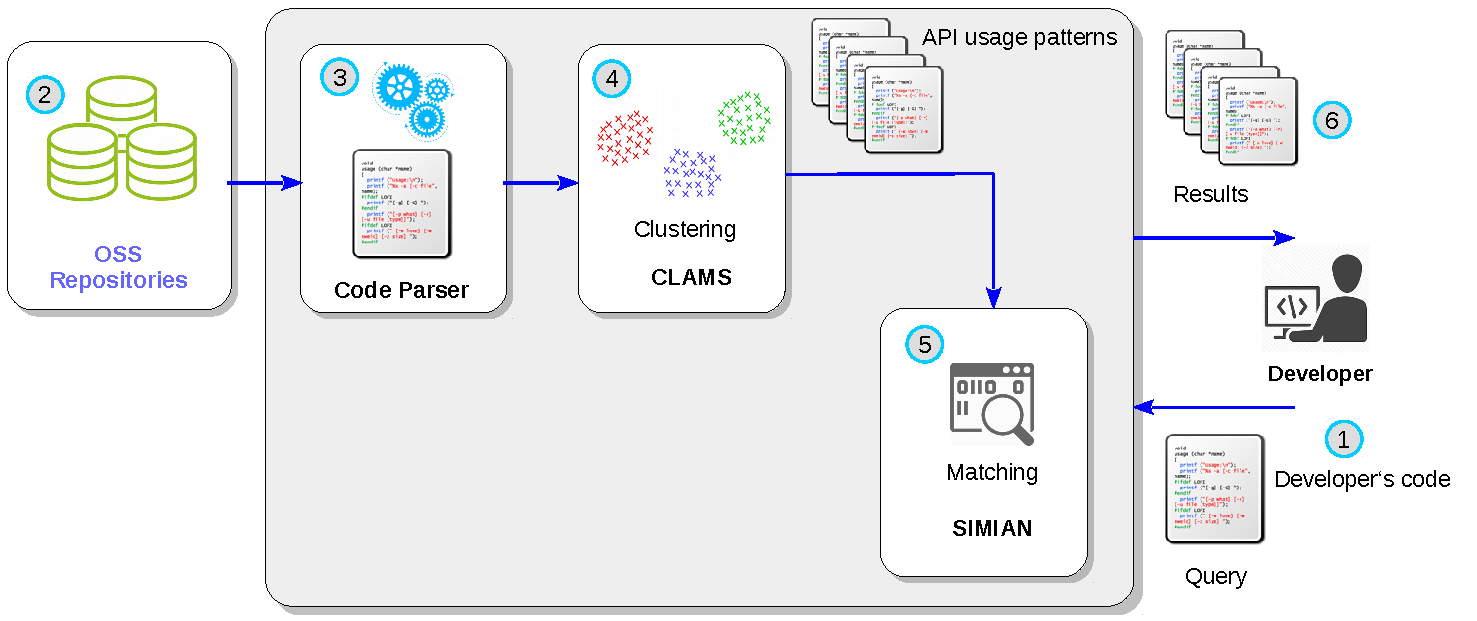
\includegraphics[width=0.80\textwidth]{images/APIUsagePatternSimianCLAM.pdf}
	%	\vspace{-.5cm}
	\caption{API usage patterns recommendation using CLAMS and Simian}	
	\label{fig:APIUsagePatternSimianCLAM}	
\end{figure}


%\begin{figure}[!h]
%	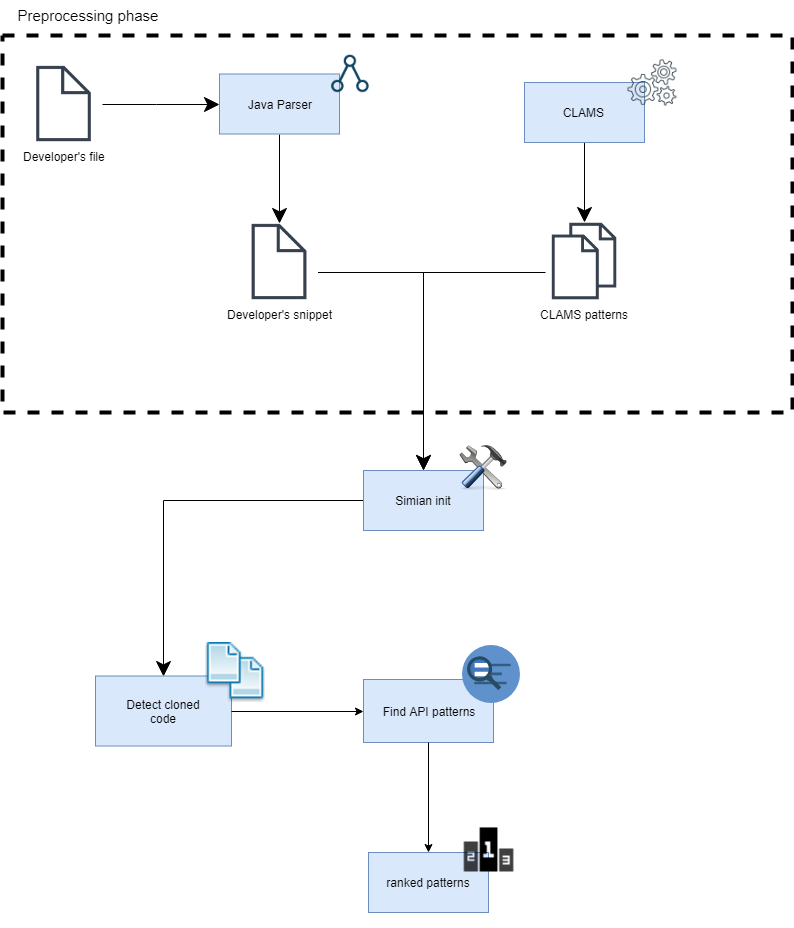
\includegraphics[width=14cm,height=16cm,keepaspectratio]{images/simian.png}
%	\centering
%	\caption{Overview of the proposed approach}
%	\label{Figure 5}
%\end{figure}

% and, furthermore it offers a solution only in the short term period


\section{Code cloning taxonomy} \label{sec:CodeClone}

To support recommendations, we choose an approach that involves code cloning 
analysis. When we analyze a software complex system, it is quite common to encounter duplicated lines of code, especially in big projects. This is done by the copy and paste technique, since it offers an 
easy solution to the current problem that the developer is facing, thus helping save time. Although this works in theory, it is not the best solution because the cloned code might bring some unexpected side effects on the other parts of the 
software. 

%Although this behaviour is discourage in general, many techniques is based on find the clones without removing them. \\
The purpose of clone cloners is to analyze software complex system in order to find the common parts among them. During the analysis, it is also important to clarify how the code has been compared and what the word cloned really means. Two fragments of code could be declared clones also if they are not exact duplicate but even if they share most of the structure (such as variable name, statement, and method calls). So, a code cloning tool must analyze also the structure, the AST and the token composition, plus the textual plain code. There are several techniques in the code cloning field, and the work by \emph{Chanchal et. al}~\cite{chanchal_k._roy_comparison_2009} provides a clear overview on this topic. In general, a clone detector tries to find the similarities between two fragments of code. Such an analysis depends first of all on the level of details that the tool wants to reach. For example, each code cloner could specify a different similarity function in order to set the level of cloning. They differ also in terms of the comparison of two snippets of code, such as AST, textual comparison, etc. There are a lot of concepts and techniques and Table \ref{tab:CodeCloningTaxonomy} depicts a taxonomy to classify the activity of code cloning.

\begin{table}[!h]
	\begin{tabular}{|p{3.2cm}|p{10cm}|}\hline
		\textbf{Code cloner type} & \textbf{Level of similarity}  \\	\hline
		Type-1 & The code fragments differs only from the white spaces, comments ad layout \\\hline
		Type-2 &  Two code fragments are syntactically equal except for the same conditions of Type-1 plus identifiers, literals and name variables\\\hline
		Type-3 &  This kind of clone detector looks for variation (add, delete or change) in statement that appears in the fragments, plus the previous conditions \\\hline
		Type-4 &  We have this kind of cloner when the computation that the fragments perform are equal without considering the syntactic implementation \\\hline		
	\end{tabular}		
	\caption{ Code cloner tools taxonomy}
	\label{tab:CodeCloningTaxonomy}
\end{table} 



%Although there exists a huge number of cloning tools and techniques, there is a common clone detection process that needs to be considered. Even using any tool, the computation may become a big issue if the common part among fragments is unknown at the beginning of the process. So, the authors identify an overall process to approach the code cloning activity, even all the steps are not required depending on the situations. The preprocessing phase, first step, is necessary to discard useless elements in the fragments of code like embedded code that appears in some language and to obtain the source units. These units can be very different depending on the purpose of the cloner and sometime they can be partitioned again in comparison units, depending on the structure of the original source unit (the common case is when we have an if-else structure in which the comparison units could be the different branches). 

%After the preprocessing, if the code cloner go further the textual analysis, a transformation phase is required, to bring all the fragments to a common representation. Among the possible normalizations that we can apply to code fragments, we have the removal of white spaces and comments, the normalization of identifiers (for example, through order sensitive index scheme), pretty-printing that affect the layout and structural transformation (for example, by removing the modifiers in a particular language). When we have a comparable units, a different comparison algorithm is run depending on the tool in order to obtain the list of matches. In this phase, we have to distinguish the fixed-granularity tools, in which the units that belongs to same block have the same granularity from the free-granularity ones in which the aggregation continues until a threshold value is reached. The list of candidates for the comparison are usually source coordinates that must be map on the original source code files. The last step is a post-processing in which clones are ranked or filtered depending on the aim that the tool wants to reach. This phase can be done by human evaluator or through a parametric heuristic algorithm. The picture below summarizes the entire procedure:


\begin{figure}[!h]
	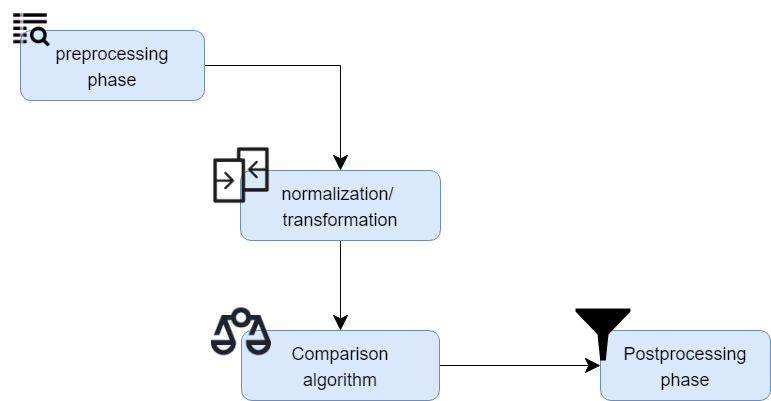
\includegraphics[width=14cm,height=14cm,keepaspectratio]{images/codeCloning.png}
	\centering
	\caption{Typical code cloning phase}
	\label{fig:CloningPhases}
\end{figure}

%Looking now to the different tools, most of them rely on different approaches to identify cloned code.


The most common code clone detecting approach is matching textual content, as the transformation and normalization phases are often very slight. The fixed lines used in the comparison are called window and they are encoded with a hash function. To obtain fragments with different lengths, the tool apply simply a slicing on the window. The lexical approach, instead, works on the tokens obtained from the source code through the compiler-style lexical analysis. This technique is more robust because it avoid the whitespaces and other dirty code that we want to exclude from the comparison. The big issue of this approach is that it not consider the syntax; so, the founded clones may overlap different syntax units but preprocessing or postprocessing can avoid this situation, like pretty-printing techniques to format the code in a better way.

%Go further, we now look at the syntactic approaches, that usually rely on the AST of the code. There are two main process  that we can apply: the tree matches and structural metrics. The first relies only on the AST extracted from the code and the comparison takes place on the subtrees. Each element of the source code(variables, literals) became a leaf of the tree and subtrees that are hashed into buckets in order to reduce the number of comparisons that take place in each bucket. However, the complexity of this approach is very high and recently there are code cloner that try to mitigate this drawback by serialize the AST as node sequence in order to reach the same speed in the same way of token based techniques. The second approach  exploits the AST is based on structural metrics. This technique avoid the direct comparison between ASTs by collecting a vector of metrics, usually calculated through fingerprints functions that consider classes, methods and statements for the metrics. The last approach that we look is the semantic technique that relies on static program analysis to provide more information rather than the syntactic one. With respect to the other approaches, the source code is represented by a PDG (Program Dependencies Graph) to keep trace the data dependencies among expression and statements. So in this case, the comparison of the clones turns to the problem of finding isomorphic subgraphs. Finally, in the literature we can find hybrid approaches that involves both syntactic and semantic analysis.

%This work includes also a very useful tool comparison, in which the authors 
%show a list of code cloners and their main features. This state of the art is 
%done by taking into account several parameters and metrics, like availability 
%of the tool, IDE integration, comparison algorithm, kind of granularity, pre or 
%post processing, language support, subsystem, possible empirical validation and 
%overall complexity. However, it is not easy to evaluate code cloning tools, 
%because there are several factors and hypothesis to taking into account when we 
%do the comparison. As we have seen, each code cloner have its own techniques, 
%comparison algorithm, approaches, complexity and supported languages, so the 
%risk to do an unfair comparison is concrete. To avoid this situation, the 
%authors set a list of possible scenario that analyze different kind of 
%situations in which the code cloning activity may be useful. \\
%The evaluation analyzes the results and if the considered code cloners are able 
%to detects the common part in particular duplicated snippet of code. There are 
%two type of scenario that the authors consider in the evaluation: the first 
%type is more technical and it considers the changes at the level of code, 
%taking as example functions that implements some features. The second type of 
%scenario involves more a not expert domain user and it focuses on the 
%intentions rather than directly on the features. For the first type of 
%scenario, we have several functions that implement a very simple mathematical 
%operation. By the copy and paste activity in which literals, variables and 
%statement change from one scenario to another, the authors look for the code 
%cloners that are able to detects these changes. Some scenarios also take into 
%account the changes that happening in the code like addition or deletion of 
%lines of code. In the second scenario, instead, a user claims the functionality 
%that he wants to realize or how many clones in the code the cloner found. 



\section{Code cloners: techniques and features} \label{sec:CodeCloners}

%After the code cloning taxonomy, useful to give a general but exhaustive idea about the code cloning domain,

In this section, we introduce some code cloners that use first track the cloned code and then return the results back to the developer. Among the techniques, we focus on the string matching one, as it is closer to the code snippets used in our approach. By this technique, there are many important issues that need to be taken into account as suggested in~\cite{stephane_ducasse_effectiveness_2005}. First of all, it is necessary to avoid false positive, \ie the part of code that is marked as duplicated but is actually not.%, that appears when the code cloner is not able to detect the cloned code during the analysis.

Moreover, scalability plays an important role since a code cloning tool must analyze complex software system which grows exponentially in recent years. An highly related issue is also the analysis of multiple languages: a good code cloner, should be able to recognize the cloned code beyond different syntaxes and lexical differences among the various programming languages. %Then, the authors propose their approach, based on the lexical analysis, following the Bellon's case study about the code cloning. In this framework, the author categorizes the clones into three types: the exact clones (Type 1), the part of code that differs from each other for the identifiers (Type 2) and clones in which statements or expressions have been inserted, deleted or changed (Type 3). This case study provides also a measure to detect how a clone is far from an other, in term of the distance. Before proceeding with the tracking activity, the authors make also the so called noise elimination on the source files that contain the cloned part to find. The noise elimination, according to the implementation done by the authors of the article, is similar to the token normalization mentioned in the taxonomy part: they remove all black spaces, comments and blocks that are not useful for the comparison.

%This phase is necessary to avoid false negative. Once they have done this normalization, they can apply the string matching techniques, based on a line by line comparison in which they look for duplicated code. From their experience, it is very difficult to find an exact code, following the definition of the Bellon'work; it is most probable to find the duplicated code among the code fragments with some modification, like insertion or deletion of statement, variable and so on.

Finally, the apply some filters on the results, as the single line is not 
enough to be significant for the cloning analysis. Therefore, they set two 
metrics, one related to minimum length sequence of the duplicated part, and the 
second related to the maximum gap size, measured between two compared 
sequences. To improve the recall of the results, they also set up a second 
normalization based on regular expression and they test the overall approach on 
the same dataset of Bellon's study, composed by the Cook and Weltab 
application. 

%\\

%Another interesting approach for the code cloning is showed in~\cite{nils_gode_incremental_2008}, in which the author proposes a code cloner with multiple revision of the code. In this way, the analysis takes 
%place not only on the original code but also on the fragments already 
%processed, in order to give a more accurate analysis. For this purpose, he 
%develops the IDA tool (Incremental detection algorithm). It is based on tokens, 
%a sequence of characters with a collective semantic, and on suffix trees, 
%already mentioned before. In particular, for the token the author use a 
%multiple token table as data structure, in order to avoid the problems that 
%arise during the multiple revision task. In facts, during the analysis tokens 
%already analyzed by the tool must be discarded from the next phases and this 
%could be left holes in the table, with a consequent overhead in the basic 
%operations like the access to data. So, when a new fragment of code is 
%analyzed, a related token table has been created to speed up the operation. 
%Also the suffix tree is affected by these side effect and the IDA tool uses a 
%generalized suffix tree to solve these issues. \\

%\newpage

%In this version, the suffix tree has multiple strings instead of one. The main 
%advantage is the speed of the operations like deletion or update of a single 
%leaf. Similar to the token tables, the fragment of code already analyzed is 
%deleted from the tree. Considering also the clone pairs, IDA integrates all 
%these components in order to make the multiple revision of code. The process 
%starts with a preprocessing phase in which IDA sets up the necessary data 
%structure in and reads the source files from the directory. Once this initial 
%phase ends, the tool starts to build the token tables and the corresponding 
%edges and nodes in the suffix trees when it is processing new files; reversely, 
%it deletes the nodes of external edges that represents the deleted files. The 
%approach is tested on three open source software, wget for downloading files, 
%gcc compilers and the Linux kernel. \\
%The last example that we show is related to Cren~\cite{jablonski_cren:_2007}, a 
%code cloner specifically developed for IDEs. In particular, the author set up 
%our tool for Eclipse platform, going further with respect to the related 
%Eclipse features, like refactor or  find and replace. The issues to face in 
%this field are mainly related to copy and paste that the a typical user do to 
%integrate into an IDE another methods or function. Reversely with respect with 
%other approaches, that use heuristic algorithms often very complex, the authors 
%of Cren provide a simpler but  effective solution in the IDEs context. 
%The core of the approach is represented by a tracking of cloned part, followed 
%by consistent rename of variables, that is the typical behaviour of a developer 
%when he tries to reimplement an API component. By exploiting the JDT features 
%related to the AST of the code, Cren is able to find not only the cloned pairs 
%but also a clone groups, represented by a sequence of two or more elements. 
%Variables and identifiers that share some characteristics are inserted in a 
%same group. Once it found the clones, it can show to the user what are the 
%cloned part in the context and, thanks to Eclipse interface, it is able to 
%highlight the cloned pairs that change dynamically with respect to the context. 
%\\
%In this way, the user can refine also the search of the cloned parts, as Cren 
%keeps trace about the cloned part already founded. Cren represents an 
%interesting mix between the code cloning technique and the IDE context. After 
%this overview about the taxonomy of code cloning and some examples of code 
%cloner, focused in particular about the suffix tree technique and an 
%incremental code cloner, we will see in the next section the code cloner chosen 
%for the implementation of our proposed approach. 







\section{Simian: A code clone detector} \label{sec:Simian}

As already mentioned in Chapter \ref{sec:Introduction}, it is possible to perform recommendation at different levels of abstraction, \eg pattern, documentation, code snippets in order to give complete and useful suggestions to developers. In our approach, the overall idea is to perform API recommendation at the level of code snippets that represent the patterns related to the developer's file. To do this, we exploit the code cloning analysis presented in the previous section. We choose Simian, a project developed in Java that performs code analysis for many languages such as Java, C, C\#, Ruby, JavaScript, to name a few. Following the taxonomy in Table \ref{tab:CodeCloningTaxonomy}, Simian is a Type-2 code cloner with flexible options on variables, literals, modifiers. All possible options are described in Table 3, although we discard some options that are related to languages different from Java, such as C. 

To test the main functionalities of the tool, we run a jar file available on the website~\cite{https://www.harukizaemon.com/simian/_last_nodate} by specifying options and the input file. As output, we get on the console the textual representation of source coordinates that describe the number of duplicated lines and the original source files. It is possible to change the type of output using the formatter option (in Table 3). As mentioned in the tool classification, Simian has the following features: 

\begin{itemize}
	\item It supports object oriented and Web languages;
	\item There are no constraints regarding any additional tools or dependencies;
	\item It is language and platform independent;
	\item It has free granularity and it analyzes line by line for each source file;
	\item It exploit fingerprint techniques for code representation;
	\item It applies transformation on variable, types and literals using options.
\end{itemize}

Among the main drawbacks, Simian does not include IDE supports and one has to do a manual integration which is going to be discussed in the next section. Moreover, it doesn't include any pre-processing or post-processing phases as well as an heuristic algorithms for the threshold or an aggregation phase at the end of the process. Also there is no specific evaluation regarding the algorithm complexity. %In particular, Simian is able to find 141,070 duplicate lines of code in 2,406 files in less than 5 seconds, that means about 28 lines of code for each second. 

Table 4 describes a very simple scenario in which we pick four pairs of Java project with the description of their main features and how lines of code are in common.

\begin{center}
	\begin{table}[!h]
		\small
		\begin{tabular}{|l|p{4cm}|p{6cm}|}\hline				
			\textbf{Option name} & \textbf{Default value} & 
			\textbf{Description} \\	\hline
			-threshold & 6 &This option fix an lower bound on the number   
			of duplicated lines of code (if present)  \\\hline
			-formatter &  none , possible values: plain, xml, emacs,    vs 
			(visual studio), yaml, null &   This option is used to obtain 
			results in a specified format\\\hline
			-reportDuplicateText & disable , type + to add &   With this 
			option, the duplicated lines of code  present in all projects 
			are printed on the console    \\\hline
			-language & disable , type + to add &  This option specifies the language of the input files to compare   \\\hline
			-defaultLanguage & disable , type + to add &   If the file type 
			is not specified, Simian inferred the type and set it as default    \\\hline
			-failOnDuplication & able , type - to remove & If this option is enabled, it causes an exception when the checker finds duplicate code     \\\hline
			-reportDuplicateText & disable , type + to add & With this 	option, the duplicated lines of code present in all projects are printed on the console    \\\hline
			-ignoreRegions & disable , type + to add & It ignores block in region structures (only for C\# programming language)  \\\hline
			-ignoreBlocks & disable , type + to add &  It excludes specified blocks from the comparison (start/end line must be specified  \\\hline
			-ignoreCurlyBraces & disable , type + to add & The curly braces are ignored  so it should be match as duplicate line \\\hline
			-ignoreIndentifier & disable , type + to add &   With this option, the variable with different identifiers match as equal 	\\\hline
			-ignoreIdentifierCase & able, type - to disable &  This option doesn't consider the case of identifiers present in the code: so Name and name are considered equal \\\hline
			-ignoreStrings & disable , type + to able &  This option considers all strings in the comparison and doesn't care about the form \\\hline
			-ignoreStringCase & able, type - to disable & Same as the previous option but considers the upper and lower case the same \\\hline
			-ignoreNumbers & disable, type + to add &   This option considers different numbers as equal  \\\hline
			-ignoreCharacter & disable, type + to add &   With this option, all character type are marked as equal  \\\hline
			-ignoreCharacterCase & able, type - to disable &  Same as ignoreStringCase but considers char by char \\\hline
			-ignoreLiterals & disable, type + to add &   All literals should be seen as equal for Simian  \\\hline
			-ignoreVariableNames & disable, type + to add &   This option allows Simian to see different variable names as equal \\\hline
			-ignoreModifiers & able, type - to disable &   This option doesn't consider modifiers of methods  (public, private, protected as element of  diversity in the code)\\\hline				
		\end{tabular}			
		\caption{ Simian options used in the experiment}
		\label{Table:3}
\end{table} 
\end{center}


\begin{table}[!h]
	\small
	\begin{tabular}{|l|p{5cm}|p{3cm}|}	\hline
		\textbf{Projects name} &  \textbf{Main features}  & \textbf{Similarity level (duplicated LOC)}  \\\hline
		ADTPlugin, ModiscoPlugin   &  Plugin projects created with same wizard & 39 lines of code in common \\\hline
		CyberGea, NeoEMFExample &   Very different projects that realize different features & No lines in common \\\hline
		CyberGea, Scuna project & The projects share only database part & 12 lines on common  \\\hline
		Simple Servlet, ServletSession &  Web projects with servelts & 35 lines of code in common  \\\hline
	\end{tabular}
	\caption{ Projects considered in the comparison }
	\label{Table:4}	
\end{table} 



From the scenario, we can see that similar projects share more common lines of code, like the first two pairs that are both Eclipse plugin projects. This happened because these projects are built with the same wizard procedure and share the initialization phase of the plugin, such as the activate method. The second pair of projects, instead, doesn't share any lines because the CyberGea project is another plugin projects that uses Mqtt paho client and JDBC libraries mainly while the Neo EMF project is related to construct a metamodel with the aim of creating a Neo4j database. Then, we compare Cybergea with another project developed in this university, the Scuna project that involves Swing framework and the MySql library for Java. It is worth noting that in this case, the two projects
share only the latter part and there are few lines in commons. 

The last example is related to Java Servlet in the Web context and Simian analyzes two kinds of servlet, one without and the other with the handling of session. The tool is able to detect the lines in common, as the servlet shares the initialization part in common like the doGet and doPost methods. All the projects shown in this simple comparison are developers in the context of university projects and their aim is only to show an example of the code cloning activity of Simian. As an additional remark, for this comparison we use the default options for Simian and launch it from the console.%, again just to give the taste of the kind of analysis that we will perform at deeper level for the proposed approach. 
 
Before going in deep in the explanation of our approach, we recall some existing approaches that deal with the problem of API recommendations.%, considering different techniques and contexts.


\section{Simian within Eclipse platform}

Once the input has been defined, there is another step in order to use Simian for API recommendations: it is necessary to integrate with the Eclipse platform to have a more flexible and usable version of the tool, as Simian doesn't support IDE integration. As already mentioned in the Related Work section, the basic version of Simian is a jar file launched from the terminal console with different options (see the Table 3). Although it is easy to use, this version is not very suitable for our purposes. To keep the integration with a Maven project, we create a repository that contains an update version of this jar and put it as reference in the \emph{pom.xml} file of the project. The following main classes need to be set: 

% and it is necessary to integrate directly the Simian jar file, available on Simian website. In order to integrate Simian in an Eclipse project, we have to set t

\begin{table}[!h]
	\begin{tabular}{|p{3.0cm}|p{10.4cm}|}\hline
		\textbf{Simian class} & \textbf{Description} \\\hline
		Auditstener &  This class is needed to initialize Simian and collects all notifications from events that occur \\\hline
		Block &  This class represents the duplicated block of code as an object and we can interact using method utilities \\\hline
		FileLoader &   It is used to load all files for the comparison, with the method load \\ \hline
		Checker &   This class is used to perform the real comparison by calling the method check() on preloaded files \\\hline
		StreamLoader &   Once we load files and create the Checker, this class loads them into the Checker \\\hline
		Options &   A data structure that encapsulates all options enabled for the comparison \\\hline
		Option &   This class represents a single option and we can specify it by accessing to a static field \\\hline
		Language &   This class contains static fields  to set all supported languages as type of input files \\\hline
		CheckSummary &  It contains all statistical data such as cloned code,  number of total files, requested time and duplicated files \\\hline
	\end{tabular}
	\caption{Overview of the classes of Simian}\label{Table:4}
\end{table} 

The project has the following structure, divided into different sub-packages:

\begin{itemize}
	\item business: it contains all the interfaces that expose the utility functions;
	\item business.impl: It contains the classes that implement the interfaces and represents the business logic of the entire application;
	\item model: It contains the representation of the SimianPattern object which is useful to keep all information for the cloning phase;
	\item evaluation: It contains all the functions necessary for the evaluation framework, specified in the proper section.
\end{itemize}



%Going in deep on the business implementation, we have 

There are three main classes as follows. SimianDataExchangeImpl collects all data needed for the analysis; SimianFileUtilitiesImpl contains all the operations related to files; and ApiCallRecommenderImpl takes all information provided by these two classes and performs recommendations. In particular, SimianDataExchangeImpl implements the original Simian class shown in the table above and it initializes the tool in order to perform the code cloning activities. Among the implemented methods, we use the function \textit{block()} to retrieve all necessary information for a duplicated block of code and the file that contains it. The \textit{endCheck()} function is called at the end of the process and manipulated the class CheckSummary mentioned before. In this way, we can obtain all information the total number of analyzed files, the duplicated ones, the time required for the comparison and the total number of blocks. This class implements also the ExchangeData interface, that is used as a bridge for ApiCallRecommenderImpl class, as the Simian interface provides only void methods without the possibility to return the necessary information.

We describe the APICallRecommenderImpl class, that collects the data coming from the previous class and analyzes them in order to produce the recommendation. The main function is \textit{findPattern()} that loads the necessary files and launches Simian analysis by exploiting the Aulistener interface. The files are loaded in pairs, in which we have the snippet of code coming from the developer's file and the other component is the list of CLAMS pattern. During the analysis phase, it is necessary to check the files and in particular, we have to discard from the analysis the files that contain duplicated blocks within themselves. It is possible because Simian retrieves for each pair the files that contains a duplicated blocks of code and, in this way, we can reduce some bias. This leads to the fact that in the developer's snippet we can have some duplicated lines of code that are not useful for the recommendation. Once we have the block, it is possible to create the object SimianPattern that represents the discovered pattern for the snippet among the CLAMS results.

The class for this object belongs to the model sub-package, that represents the extracted pattern. Following the POJO structure, we have the \textit{getter} and \textit{setter} functions for each property of the object, gradually filled during the analysis. We have duplicated lines to store the cloned code, the filename of the pattern and the elapsed time for each pattern that Simian has found in the analysis. In this way, we can easily write to a file to show the final results in a more comprehensive way. The original Simian output, in facts, shows only the duplicated lines and CLAMS puts the patterns in a ranked list but without the context, represented in this case by the import at the beginning of the file. Thanks to this structure, we can also rank the patterns from the one that have more lines in commons, using the proper field in the wrapper class.

The last main component is SimianFileUtilities, in which we open all necessary files, write the recommendations and create temporary files for the code cloning activity. All these classes are integrated in test class that calls in the proper sequence all the methods to perform the final recommendation. In particular, the method \textit{scan()} takes all files that contain patterns extracted by CLAMS while the function \textit{createTemporaryFile()} creates the temporary files to perform the comparison. To extract the ground truth part used in the evaluation part, we use \textit{parseAST()}. This function uses the JavaParser library to traverse the AST and take the body of the method that we are interested in. In this way, Simian inputs are only partial fragments of code that represent the typical developing scenario. 

The project contains also classes with the evaluation task, such as the function to build the Rascal project structure in order to analyze the corresponding method invocations and to apply the metrics on them. More details are going to be provided in the evaluation framework section. The overall architecture is depicted in Figure \ref{fig:ComponentDiagram}.

\begin{figure}[!h]
	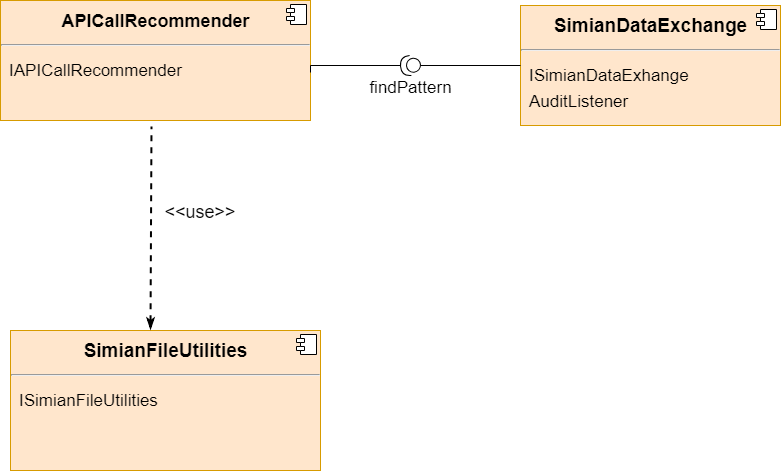
\includegraphics[width=12cm,height=12cm,keepaspectratio]{images/Component.png}
	\centering
	\caption{Component diagram}
	\label{fig:ComponentDiagram}
\end{figure}








\section{Preprocessing}

The input files that are necessary to initialize the tool, we have from one side the developer's file with the real snippet of code that she is implementing and needs support for this. From the original file, we extract a portion that represents the context of the recommendation that can be a list of method invocations or simply a list of variable declarations. This portion is called ground truth and it is the part used as the context of the recommendation. On the other hand, there are patterns mined by CLAMS, in the form of ranked Java files sorted by rational specified in CLAMS paper. These files contain patterns, defined as a sequence of API method calls that define, instantiate class belonging to the APIs contained in the developer' string. The number of the files and also their dimensions in term lines of code depends on the considered libraries. As Simian is a tool based on file comparison, we use temporary files of Java to do the comparison, after the process, the files are discarded to save memory. 

This preprocessing phase is required as mentioned in the Related Work section, the tool doesn't include any built-in preprocessing. To extract the snippet of code from the developer's file, we use Java Parser, an open source project that allows one to analyze, modify and generate Java code, to traverse the AST of the input files and take the body of a method randomly selected that composes our ground truth. We consider only compilable files, otherwise Java Parser is not able to build the corresponding AST for the analysis. We take into consideration only the ground truth files because we are in the typical scenario in which the developer is starting to implement some features and she has written only some code fragments. In general a recommendation relies on the context in on which the developer is working. In our case, the context is the developer's code snippet with imports and variable declarations.

For CLAMS, we create a golden set of $5$ libraries, chosen among the set of $15$ libraries available at the authors' website. For each of them, CLAMS retrieves a list of patterns represented by Java files and their number depending on the library that we consider. The precision and the lines of code of this list depend on the clients and examples files. We can also decide which methods and classes that CLAMS analyzes through the namespaces file in the proper folder. This phase is necessary because Simian doesn't have a well-defined preprocessing phase and needs to defined in a proper way. We can define the entire procedure that just describes a human preprocessing, since we don't use any automatic procedure or heuristic algorithm to select the input files. We select relevant client files, and avoid test classes. For CLAMS pattern, we don't put any limitation and we consider all possible patterns retrieved for a specific library.


%, that are too smaller for our purpose and interfaces, that haven't no relevant body
% Reversely, we don't consider an entire class or project, because in this scenario, the developer has completed almost the task and it is not interest in possible recommendations. 
%%%%%%%%%%%%%%%%%%%%%


%%%%%%%%%%%%%%%%%%%%%%%%%%%%%
%the difficulties in approaching an API, as there are many aspects to take into 
%consideration. As we will see, for the our proposed approach we used code 
%example and in particular the snippet of code to perform the recommendation, 
%trying to avoid the above issues related to the API such as the lack of best 
%practices and the ambiguous usage of a component. Another emerging aspect is 
%that the documentation should be clear about the design, the abstraction and 
%the features provides by the API. We don't directly work on the documentation, 
%but we try to offers a solution at level of code that could be integrate this 
%lack of information.




\section{CLAMS adaptation}

Regarding the output by CLAMS, we describe the original structure as well as the necessary modification to integrate it into our tool. The complete source code has been made available by the authors. CLAMS is written in Python and uses srcXML and Astyle to produce XML files and to formatter in a human-readable way the code respectively. As claimed by the authors, there are no specific constrains about the technologies to use in case of a new implementation. As input, CLAMS takes two kinds of files: client files that represent the real project on Github related to the dataset that authors use for evaluation phase while example files are used as training set.

All these files are collected in a folder and CLAMS loads by getting the path. Moreover, there is a namespace file that identifies the name of classes used in the clients and example files by using their complete namespaces such as org.codehaus.jackson. The last input used by the main.py file, that is used to initialize the platform, is the list of methods that are represented by an ARFF (Attribute-Relation File Format) file~\cite{https://www.cs.waikato.ac.nz_last_nodate}. It is an ASCII text file that describes a list of instances sharing a set of attributes, specified in the header section. In our case, the attributes are the method declaration (the caller) and the method invocations (the calls). 

There is a phase of preprocessing in which CLAMS extracts API calls and their AST using JDT utilities and represents them in XML using srcXML. The core of the project is the snippet generator module (represented by summarise.py file) that takes as input a source code file (Java in this case) and using srcXML they first replace literals with XML types and delete comment. Then, they separate the API code from the code that doesn't contain API calls and highlights the variable in local scope of API. Finally, the code without API call is removed and CLAMS adds some comments near the API statement and needed variables. The approach considers also the classical statement like if-else structure as a part of API statement. 

For clustering, both HDBSCAN and k-Medoids algorithms are used that differ only in the precision of the returned snipped (HDBSCAN is more accurate but k-Medoids covers more methods). The rank is based on the example files that contains a sequence of API call; if the sequence within the file is a super-sequence of the sequence of snippet that we considered, so this snippet is supported, and its rank is increased. In the result folder, CLAMS puts the library that we want to analyze, the methods, the source file (both in .java and xml format), some JSON files that represent all information about a method (class, package, rank, id) and the ARFF file related to the library.

For the integration step in our platform, it is necessary to slightly modify the original approach to have better results. In particular, if we use the pattern of CLAMS as they are, there are some bias since through srcML, CLAMS substitutes the literals with its own type and Simian is not able to detect them as cloned code, even using all available options regarding the code. To avoid this, we modify the function that substitutes literals, putting some default values instead of srcML types. This modification doesn't affect the validity and accuracy of extracted path as it is just a matter of modifying literals with another and allow Simian to avoid bias in the code cloning analysis.

\section{API recommendations}

At the end of the preparatory phases, we describe now the core of this project, the API recommendations. Once Simian is launched, it performs the detection of code cloning activity on the CLAMS patterns files and the developer's code snippet. The typical scenario is depicted by the use case diagram in Figure \ref{fig:UseCaseScenario}, in which the developer asks for recommendations.


\begin{figure}[!h]
	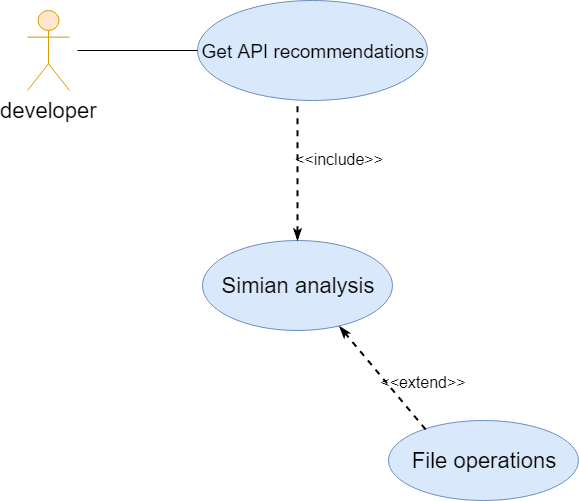
\includegraphics[width=10cm,height=10cm,keepaspectratio]{images/Usecase.png}
	\centering
	\caption{Use case scenario}
	\label{fig:UseCaseScenario}
\end{figure}



The notion of cloned code depends on the options that we have selected and turn on: the mandatory option to enable is the threshold, that sets the minimum lines of code in commons, reportDuplicateText, otherwise we couldn't show and manipulate the result and language that is Java because we analyze projects related to it. Without this options, Simian gives us only the fingerprints that represent the source coordinates of the files, which are not significant for our purpose. Thus, to have a better representation, we put the results in a wrapper class that represent the Pattern object in which we have all attributes to describe the recommendation in the right manner.

Other options, such as strings, identifiers or modifiers that should be introduced in the comparison, can be enabled with respect to the level of cloning that we want to reach. To find useful results, it is necessary to set at least ignoreIdentifiers, ignoreIdentifierCase, ignoreLiterals, ignoreVariableName, ignoreNumbers and ignoreModifiers since Simian goes beyond the developer personal implementations and looks only for the structure of the code, in order to use the concept of pattern in a more effective way. Based on these options, Simian applies the proper transformations on the original textual code in order to perform the comparison. 

Furthermore, Simian compares the pair developer's snippet - pattern because some CLAMS patterns include some duplicated lines of code and this can bring some bias. Once we load the files, the check is performed and the results that include lines of code, name of pattern file and time to perform the comparison and put all in the wrapper class mentioned before.

At the end of this step, we have the patterns (a complete one or only partial) that the developer can start to implement and we can discard it from the comparison, as the developer is not interested to see what he has done so far. The last step is to remove the duplicated lines of code from the suggested patterns and show to the developer only the new part, that integrates his code or proposes new patterns for that feature, related of course to the library that he is implementing. About the ranking, we order the pattern by considering the number of cloned lines, so the first pattern contains more duplicated lines than second one and so on. The ranking is simply performed on the SimianPattern object that we produce as output. All the steps are summarized in \ref{fig:SequenceDiagram}.


\begin{figure}[!h]
	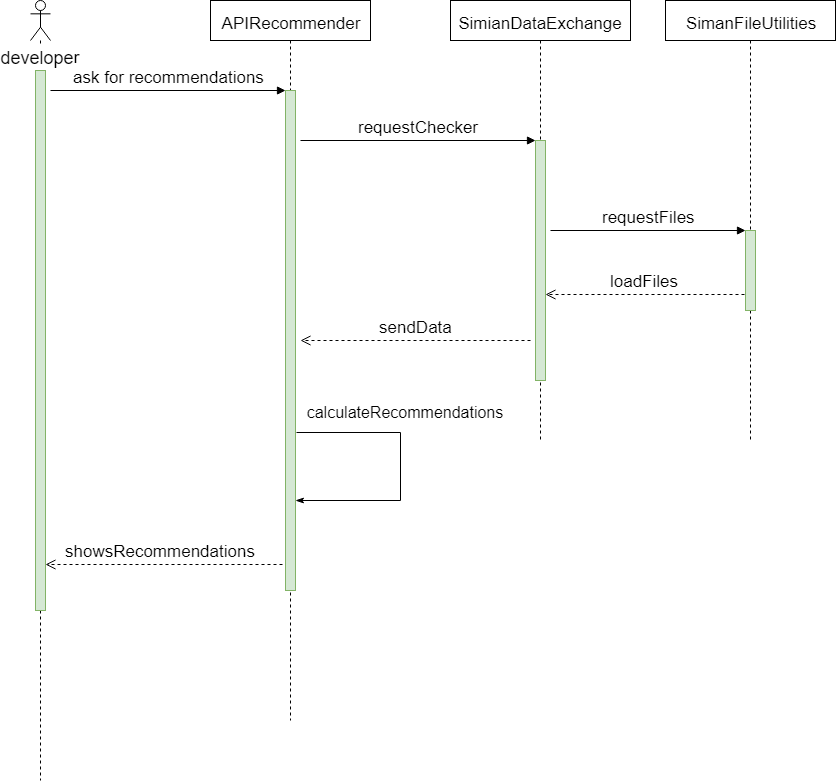
\includegraphics[width=14cm,height=16cm,keepaspectratio]{images/Sequence.png}
	\centering
	\caption{Sequence diagram }
	\label{fig:SequenceDiagram}
\end{figure}


The example below is related to the \emph{MQTT paho} library, we have extracted the method \emph{publish()} from the developer's file with Java Parser and run Simian on it. The last columns show two top rank CLAMS patterns.
\vspace{5mm}

Developer's original file
\begin{lstlisting}
package org.eclipse.paho.sample.mqttv3app;
import java.io.IOException;
import java.sql.Timestamp;
import org.eclipse.paho.client.mqttv3.IMqttDeliveryToken;
import org.eclipse.paho.client.mqttv3.MqttCallback;
import org.eclipse.paho.client.mqttv3.MqttClient;
import org.eclipse.paho.client.mqttv3.MqttConnectOptions;
import org.eclipse.paho.client.mqttv3.MqttException;
import org.eclipse.paho.client.mqttv3.MqttMessage;
import org.eclipse.paho.client.mqttv3.persist.MqttDefaultFilePersistence;

public class Sample implements MqttCallback {		
public Sample(String brokerUrl, String clientId, boolean cleanSession, boolean quietMode, String userName, String password) throws MqttException {    	
try {    		
conOpt = new MqttConnectOptions();
conOpt.setCleanSession(clean);
if(password != null ) {
conOpt.setPassword(this.password.toCharArray());
}
if(userName != null) {
conOpt.setUserName(this.userName);	   
}    		
client = new MqttClient(this.brokerUrl,clientId, dataStore);		
client.setCallback(this);

} catch (MqttException e) {
e.printStackTrace();
log("Unable to set up client: "+e.toString());
System.exit(1);
}
}

public void publish(String topicName, int qos, byte[] payload) throws MqttException {

// Connect to the MQTT server
log("Connecting to "+brokerUrl + " with client ID "+client.getClientId());
client.connect(conOpt);
log("Connected");   	
String time = new Timestamp(System.currentTimeMillis()).toString();
log("Publishing at: "+time+ " to topic \""+topicName+"\" qos "+qos);    
MqttMessage message = new MqttMessage(payload);
message.setQos(qos);     
client.publish(topicName, message);    	
// Disconnect the client
client.disconnect();
log("Disconnected");
}


public void subscribe(String topicName, int qos) throws MqttException {    	    
client.connect(conOpt);
log("Connected to "+brokerUrl+" with client ID "+client.getClientId());    
log("Subscribing to topic \""+topicName+"\" qos "+qos);
client.subscribe(topicName, qos);
// Continue waiting for messages until the Enter is pressed
log("Press <Enter> to exit");
try {
System.in.read();
} catch (IOException e) {
//If we can't read we'll just exit
}		
// Disconnect the client from the server
client.disconnect();
log("Disconnected");
}
}
\end{lstlisting}



%\vspace{5mm}
%\newpage

Extracted method:
\begin{lstlisting}

// Connect to the MQTT server
log("Connecting to " + brokerUrl + " with client ID " + client.getClientId());
client.connect(conOpt);
log("Connected");
String time = new Timestamp(System.currentTimeMillis()).toString();
log("Publishing at: " + time + " to topic \"" + topicName + "\" qos " + qos);
// Create and configure a message
MqttMessage message = new MqttMessage(payload);
message.setQos(qos);
// Send the message to the server, control is not returned until
// it has been delivered to the server meeting the specified
// quality of service.
client.publish(topicName, message);
// Disconnect the client
client.disconnect();
log("Disconnected");
\end{lstlisting}

\noindent

\begin{minipage}[t]{0.4\textwidth}
	\begin{lstlisting}
	CLAMS pattern #1
	{
	String pubTopic;
	MqttClient pubClinet;
	String payload;
	int qos;
	pubClinet = new MqttClient(url, clientId);
	pubClinet.setCallback(this);
	pubClinet.connect();
	MqttMessage message = new MqttMessage(payload.getBytes());
	pubClinet.publish(pubTopic, message);
	pubClinet.disconnect();
	}
	\end{lstlisting}
\end{minipage}
\hfill

\begin{minipage}[t]{0.5\textwidth}
	\begin{lstlisting}
	CLAMS pattern #2
	{
	String topicName;
	MqttAsyncClient client;
	MqttConnectOptions conOpt;
	String brokerUrl;
	byte[] payload;
	int qos;
	log("a string"+brokerUrl
	+ "a string"+client.getClientId());
	IMqttToken conToken = client.connect(conOpt,null,null);
	log("a string" +System.currentTimeMillis()+ "a string"+topicName+"a string"+qos);
	IMqttDeliveryToken pubToken = client.publish(topicName, message, null, null);
	pubToken.waitForCompletion();
	IMqttToken discToken = client.disconnect(null, null);
	discToken.waitForCompletion();
	}
	
	\end{lstlisting}
\end{minipage}

%\newline

In particular, the two extracted recommendations show two possible uses of the object MqttMessage that the developer declared in the publish method. The first recommendation adds an MqttClient while the second uses the interface IMqttDeliveryToken as a different way to send the \emph{mqtt} message. The number of recommendation is strongly related to the length of the method and how many lines Simian can detect in its textual analysis. This example is used just to show the expected output after running our approach. In general, given a project that uses different libraries, with this approach we are able to recommend patterns of whatever libraries that the user is interested in. As mentioned before, recommendations are at level of code snippet and provide a concrete and immediate hint. As we choose CLAMS for the second element of the clone pair, we are not able to provide tutorial or complete application as recommendation, because only patterns are available for this purpose.

We can support almost the dataset of CLAMS and different libraries like MQTT or Json. The quality of recommendations depends first of all on the blocks in the developer's file that Simian is able to detect in the patterns provided by CLAMS. Providing more patterns means more support for the library and this brings more API recommendations at the end of the process. Another aspect to be taken into account is that Simian analyses the duplicated blocks of code and maybe some methods invocations that are not in the correct sequence are discarded automatically from the final recommendation.

In the next chapter, we are going to present an evaluation framework by using part of the dataset of CLAMS (as we have already the patterns used by Simian for the comparison). We do this as a double check validation because Simian doesn't have a post-processing phase and we need a comparison that goes beyond the lexical one in order to apply the metrics. Moreover, we will be comparing the results with those generated by PAM.%, already described in the existing approach section.




